\section{Ablation}
\label{sec:ablation}

The ablation asks what each component of the estimation ladder contributes, and what the design variables of the protocol contribute, on the same histories. A component is compared with the rung just before it on the histories where both return a capital, so the comparison is paired and is not confounded by the histories on which a rung fails.

\subsection{Components of the estimation ladder}
\label{sec:abl-components}

\Cref{tab:ablation} and \cref{fig:ablation} give, for each component, the share of paired histories within a factor of two of the truth before and after, the change with its 95 percent bootstrap interval, and the standard deviation of the logarithm of the ratio.
Modelling the collection threshold lifts the share within a factor of two from \abThresholdFrom{} to \abThresholdTo{} percent, a gain of \abThresholdDelta{} points (interval \abThresholdLo{} to \abThresholdHi{}) over \abThresholdN{} paired histories: it is necessary, because ignoring it puts the median capital at \cLgATbMed{} of the truth at $\xi=0.6$ and at \cLgDTbMed{} at $\xi=1.1$, and far from sufficient.
Splicing a generalised Pareto tail onto the lognormal body adds \abHeavytailDelta{} points (\abHeavytailFrom{} to \abHeavytailTo{} percent) but increases the dispersion of the logarithm of the ratio from 0.79 to 1.52: the splice removes bias and adds variance, because the tail has two parameters fitted only on the losses above EUR 100,000, a small part of the recorded history.
Replacing the aggregation of the splice by the closed-form single loss approximation on a generalised Pareto fit above the collection threshold adds \abClosedformDelta{} points and halves the dispersion of the logarithm, because the fit uses every recorded loss above the threshold instead of the few above the splice point; this is the largest gain among the components that read only the data.
The adjustment by one mean adds \abMeanadjustedDelta{} points (interval \abMeanadjustedLo{} to \abMeanadjustedHi{}), which is small but has an interval that excludes zero. It is refused wherever the fitted index is one or more and is compared over \abMeanadjustedCells{} cells, at 1.1 only on the histories whose fitted index is below one.
The mean correction is not read as a component, because its form is not confirmed against a primary text (\cref{sec:pm-ladder}). Its row, the last of \cref{tab:ablation} and set apart there, is a comparison on the \abMeancorrectionCells{} cells where it is computed (it is not computed for the variant whose true index is 1.1): it adds \abMeancorrectionDelta{} points (interval \abMeancorrectionLo{} to \abMeancorrectionHi{}). The two corrected capitals differ by exactly one mean of the fitted severity (\cref{eq:mean-corrections}) and agree on the same history to a median of \rFiveSevenMed{} percent, so the comparison row and the adjustment are one effect in two forms and are not added.

\begin{table}[htbp]
\centering\scriptsize
\caption{The ablation of the estimation ladder: for each component, the paired comparison on the histories of the 16 cells where both rungs return a capital, the share of those histories within a factor of two of the truth before and after, the change in percentage points with its 95 percent bootstrap interval over the paired histories, and the standard deviation of the logarithm of the ratio before and after. The last row is a comparison only, on the 12 cells where the mean-corrected rung is computed: its form is not confirmed against a primary text, so it is not read as a component of the ladder.}
\label{tab:ablation}
\fitwidth{\begin{tabular}{llrrrrr}
\toprule
Component & Rungs compared & Pairs & Before (\%) & After (\%) & Change (points) [95\% CI] & $\mathrm{sd}$ of $\ln$ ratio \\
\midrule
Model the collection threshold & Lognormal, threshold ignored to Truncated lognormal & 11{,}876 & 0.0 & 14.8 & +14.8 [+14.2, +15.5] & 1.24 to 0.86 \\
Splice a GPD tail onto the body & Truncated lognormal to Lognormal-GPD splice & 9{,}385 & 13.6 & 35.2 & +21.6 [+20.4, +22.9] & 0.79 to 1.52 \\
Closed-form tail instead of aggregation & Lognormal-GPD splice to Single loss approximation & 10{,}743 & 34.0 & 59.5 & +25.4 [+24.3, +26.6] & 1.63 to 0.87 \\
Replace the tail by the scenario credibility tail & Lognormal-GPD splice to Scenario combination & 10{,}743 & 34.0 & 82.5 & +48.5 [+47.3, +49.6] & 1.63 to 0.48 \\
Adjust the approximation by one mean & Single loss approximation to Mean-adjusted single loss approximation & 11{,}337 & 58.6 & 61.6 & +3.0 [+2.6, +3.4] & 0.84 to 0.82 \\
Fit the GPD by Cram\'er-von Mises & Mean-adjusted single loss approximation to Cram\'er-von Mises GPD & 10{,}371 & 62.2 & 47.6 & -14.6 [-15.7, -13.5] & 0.81 to 1.07 \\
Fit the GPD by the bias-robust estimator & Mean-adjusted single loss approximation to Optimally bias-robust GPD & 10{,}941 & 61.7 & 60.0 & -1.7 [-2.4, -1.0] & 0.82 to 0.86 \\
Fit a lognormal instead of the GPD & Cram\'er-von Mises GPD to Cram\'er-von Mises lognormal & 10{,}275 & 49.1 & 4.9 & -44.2 [-45.3, -43.1] & 1.05 to 0.91 \\
\midrule
\multicolumn{7}{l}{\emph{Comparison only, in no count of the text (form not confirmed)}} \\
Add the mean correction & Single loss approximation to Single loss approximation, mean correction & 10{,}635 & 62.5 & 65.5 & +2.9 [+2.5, +3.4] & 0.79 to 0.76 \\
\bottomrule
\end{tabular}}
\end{table}


\begin{figure}[htbp]
\centering
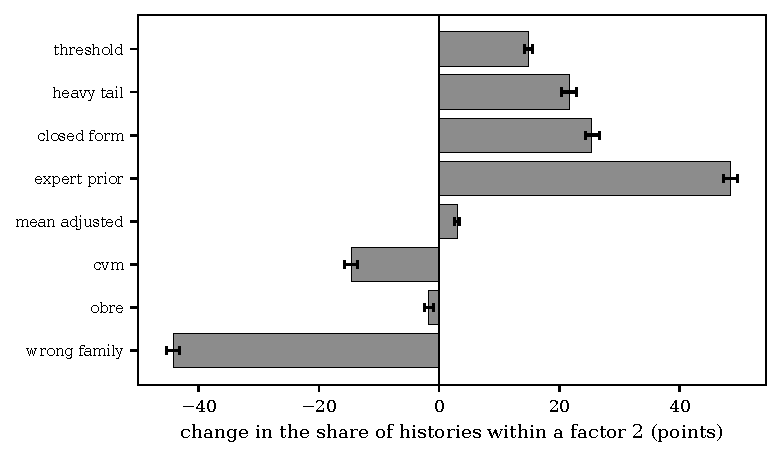
\includegraphics[width=0.78\textwidth]{ablation-change.pdf}
\caption{Change in the share of histories within a factor of two of the truth when each component of the estimation ladder is added, in percentage points with 95 percent bootstrap intervals over the paired histories of the 16 cells where both rungs return a capital; the comparison row of the mean-corrected rung is in \cref{tab:ablation} only.}
\label{fig:ablation}
\end{figure}

The scenario credibility tail adds \abExpertpriorDelta{} points over the splice, from \abExpertpriorFrom{} to \abExpertpriorTo{} percent, the largest change of the table. It is also the component that does not read the data: the prior of the Pareto shape is the expert's, the true severity quantiles of the generator rounded to two significant figures, so the gain measures what an accurate expert is worth to the estimate and not what the method extracts from a history. A biased expert would move the same rung the other way, and the experiment does not vary the expert.
The two robust fits do not help on this process. The minimum Cram\'er-von Mises fit lowers the share within a factor of two by \abCvmDown{} points (interval \abCvmDownLo{} to \abCvmDownHi{}) and raises the dispersion, as expected of a distance on the distribution function, which gives the largest losses, the ones that fix the tail, little weight, and the optimally bias-robust fit at an efficiency of 0.95 lowers it by \abObreDown{} points. The synthetic losses contain no contamination, so the protection of a robust estimator has nothing to protect against, and what remains is its loss of efficiency.
Fitting a lognormal instead of the generalised Pareto family drops the share within a factor of two to \abWrongfamilyTo{} percent: a misspecified family is the largest negative effect of the table and is not repaired by robustness.

\subsection{Length of the history and collection threshold}
\label{sec:abl-design}

Doubling the history from 5 to 10 years divides the standard deviation of the logarithm of the single loss approximation by \yrRatio{} on average over the eight pairs of cells (range \yrRatioMin{} to \yrRatioMax{}), which is the \sqrtTwo{} of the $1/\sqrt T$ law of \cref{cor:leading} to within the error of the measurement. Raising the collection threshold from EUR 10,000 to 20,000 removes between 31 and 52 percent of the median number of recorded losses (the expected numbers $k$ of \cref{tab:theory}), and multiplies the dispersion by \thrRatio{} on average (range \thrRatioMin{} to \thrRatioMax{}), in the direction and of the order that the $k^{-1/2}$ law of \cref{cor:leading} gives for the smaller number of recorded losses.
Neither variable brings any rung near the green limit, and the history that would is of the order of a century (\cref{fig:years}). The threshold is a modelling choice a bank makes, and the result says that the cost of a higher threshold is a larger dispersion even when the truncation is modelled correctly.

The two effects combine multiplicatively in the theory, so that a bank with ten years and the lower threshold has the smallest dispersion of the four cells at every tail index.

\subsection{Number of histories}
\label{sec:abl-histories}

The number of histories per cell is a component of the protocol. With 50 histories the relative standard deviation of the measured interquartile range of the splice is \subSpFifty{} percent and with 250 it is \subSpTwoFifty{}, and it falls close to the $n^{-1/2}$ law (\cref{fig:precision}); with the 1{,}000 histories of the experiment the bootstrap relative standard deviation is \bootSpMed{} percent for the splice (\bootSpMin{} to \bootSpMax{} across cells) and the intervals of \cref{tab:main-results} separate the lightest tail from the heaviest ones but, for the splice, overlap between neighbouring cells at the same tail index.

The number of histories is a cost and not only a precision. The 16 cells took about 70 minutes on ten processes, and the cost grows linearly with the number of histories while the precision improves as its inverse square root: halving the relative standard deviation of \subSpFiveHundred{} percent of the measured interquartile range of the splice at 500 histories would take four times as many histories. The number of histories is fixed by the design at 1{,}000 and no stopping rule is applied; at that number the interval of the interquartile range at the heavy tails is still wide, and the protocol reports the interval so that the reader sees the remaining uncertainty and not a point value that seems precise. A study of a single cell could draw many more histories at the cost of the other cells.
